\documentclass[11pt]{article}
\usepackage[margin=1in]{geometry}
\usepackage{amsmath}
\usepackage{booktabs}
\usepackage{graphicx}

\title{Step 6 Validation Protocol: Dynamic Phonon Parameter Scans}
\author{}
\date{}

\begin{document}
\maketitle

\section{Purpose of the test}
Steps 4 and 5 showed that the lattice-dynamic channel follows the imposed
spin-Peierls trend.  Step 6 isolates the dynamic phonon coordinate itself.  The
goal is to identify which finite-window observables scale with the operator
term $g_Q Q L_{BD}$ rather than with scalar bright-dark mixing.

\section{Physical model}
The Hamiltonian is
\begin{equation}
H_{\mathrm{mix}} =
V_{BD}^{\mathrm{static}} L_{BD}
+ g_Q Q L_{BD},
\end{equation}
with
\begin{equation}
Q=a+a^\dagger.
\end{equation}
The static component $V_{BD}^{\mathrm{static}}$ is held fixed at the
low-temperature reference value.  The scan therefore changes only the dynamic
phonon parameters:
\begin{equation}
g_Q \quad\mathrm{or}\quad \omega_Q.
\end{equation}

\section{Expected results}
The $g_Q=0$ case is the static scalar reference.  Increasing $g_Q$ should
change at least one finite-window observable relative to that reference:
cross-window area, cross/diagonal ratio, sideband/main-cross ratio, full
spectrum norm, or pathway-resolved amplitude.  For sufficiently weak coupling,
changes in intensities are expected to be approximately even in $g_Q$ because
the spectrum is insensitive to the sign of a single harmonic displacement in
many aggregate observables.

The $\omega_Q$ scan should affect windows displaced by $\pm\omega_Q$.  If the
dynamic sideband interpretation is useful, the sideband-sensitive metrics
should vary with $\omega_Q$ even when $V_{BD}^{\mathrm{static}}$ and $g_Q$ are
held fixed.

\section{Numerical procedure}
Run one parameter set at a time using \texttt{STEP6\_ACTIVE\_CASE}.  The
recommended cases are:
\begin{center}
\begin{tabular}{ll}
\toprule
Scan & Values \\
\midrule
$g_Q$ & 0, 0.0025, 0.005, 0.010, 0.015, 0.020 \\
$\omega_Q$ & 0.020, 0.035, 0.050, 0.070 eV \\
\bottomrule
\end{tabular}
\end{center}
The pulse sequence and NQ protocol are the same as in Step 5: third-order 1Q
rephasing spectra with the standard pathway set.  The frequency grid is wide
enough to include the bright/dark resonances and nearby phonon-displaced
windows.

\section{Acceptance criteria}
The $g_Q$ scan passes if the $g_Q=0$ static reference is distinct from at least
one nonzero-$g_Q$ spectrum in a finite-window metric or full-spectrum norm, with
$V_{BD}^{\mathrm{static}}$ unchanged.  It is inconclusive if all nonzero values
look identical to the static reference within numerical tolerance.

The $\omega_Q$ scan passes if sideband-sensitive metrics vary with
$\omega_Q$.  It is inconclusive if the metric is dominated by tails from the
main resonances or by finite-window placement rather than by the phonon energy.

\section{Requested figures and data}
For each run, save:
\begin{itemize}
\item the rephasing real spectrum PDF;
\item pathway-resolved complex response arrays;
\item total rephasing, unrephasing, and 1Q components;
\item text and JSON summaries containing $V_{BD}^{\mathrm{static}}$, $g_Q$,
$\omega_Q$, and the finite-grid settings.
\end{itemize}
Phase 2 should produce scan tables, trend plots for $g_Q$ and $\omega_Q$, and a
validation outcome file.

\section{Interpretation of possible failures}
If the $g_Q$ scan produces no clear change, the coupling may be too weak, the
phonon basis may be too small, or the chosen finite windows may be insensitive
to the dynamic coordinate.  If the $\omega_Q$ scan does not move or change the
sideband metrics, the observable may be dominated by the main resonances rather
than by genuine phonon-displaced pathways.

\section{Numerical results}
The Step 6 scan generated ten spectra at $\eta=0.001$ on a $120\times120$
frequency grid.  Throughout this test,
$V_{BD}^{\mathrm{static}}=0.02$ was held fixed, so the observed changes are not
caused by scalar bright-dark mixing.  The finite-window half-width was
$0.025$ eV.

\begin{center}
\begin{tabular}{rrrrr}
\toprule
$g_Q$ & $A_{\mathrm{cross}}$ &
$A_{\mathrm{cross}}/A_{\mathrm{diag}}$ &
$A_{\mathrm{side}}/A_{\mathrm{cross}}$ & $\|S_R\|_2$ \\
\midrule
0 & 16.266623 & 0.127003 & 2.329115 & 1196548 \\
0.0025 & 15.927155 & 0.127904 & 2.344188 & 1144065 \\
0.0050 & 14.997807 & 0.130900 & 2.389604 & 1000153 \\
0.0100 & 12.554241 & 0.145423 & 2.549178 & 622490 \\
0.0150 & 11.978064 & 0.170810 & 2.468308 & 442198 \\
0.0200 & 18.471655 & 0.201674 & 1.982344 & 776222 \\
\bottomrule
\end{tabular}
\end{center}

The $g_Q$ scan clearly changes the nonlinear response even though the static
mixing is fixed.  The full rephasing norm changes by relative amount
$6.30\times10^{-1}$ compared with the $g_Q=0$ static reference.  The
cross/diagonal ratio increases monotonically from $0.127003$ to $0.201674$.
The main cross-window area and full norm are not monotonic: both decrease up to
intermediate coupling and then increase at $g_Q=0.020$.  This nonmonotonicity is
not a failure; it indicates that the dynamic phonon coordinate changes the
spectral redistribution rather than acting as a simple scalar amplitude.

\begin{center}
\begin{tabular}{rrrrr}
\toprule
$\omega_Q$ & $A_{\mathrm{cross}}$ &
$A_{\mathrm{cross}}/A_{\mathrm{diag}}$ &
$A_{\mathrm{side}}/A_{\mathrm{cross}}$ & $\|S_R\|_2$ \\
\midrule
0.020 & 13.137004 & 0.134156 & 3.378482 & 803047 \\
0.035 & 12.554241 & 0.145423 & 2.549178 & 622490 \\
0.050 & 11.581389 & 0.155038 & 2.266216 & 478460 \\
0.070 & 11.157339 & 0.160376 & 3.141335 & 441798 \\
\bottomrule
\end{tabular}
\end{center}

At fixed $g_Q=0.010$, increasing $\omega_Q$ reduces both the main cross-window
area and the full rephasing norm, while the cross/diagonal ratio increases.  The
sideband/main-cross ratio varies with a relative spread of
$3.29\times10^{-1}$, passing through a minimum near $\omega_Q=0.050$ eV.  This
metric is sensitive to $\omega_Q$, but it should be interpreted qualitatively
because finite sideband windows can include tails from nearby resonances.

\begin{figure}[h]
\centering
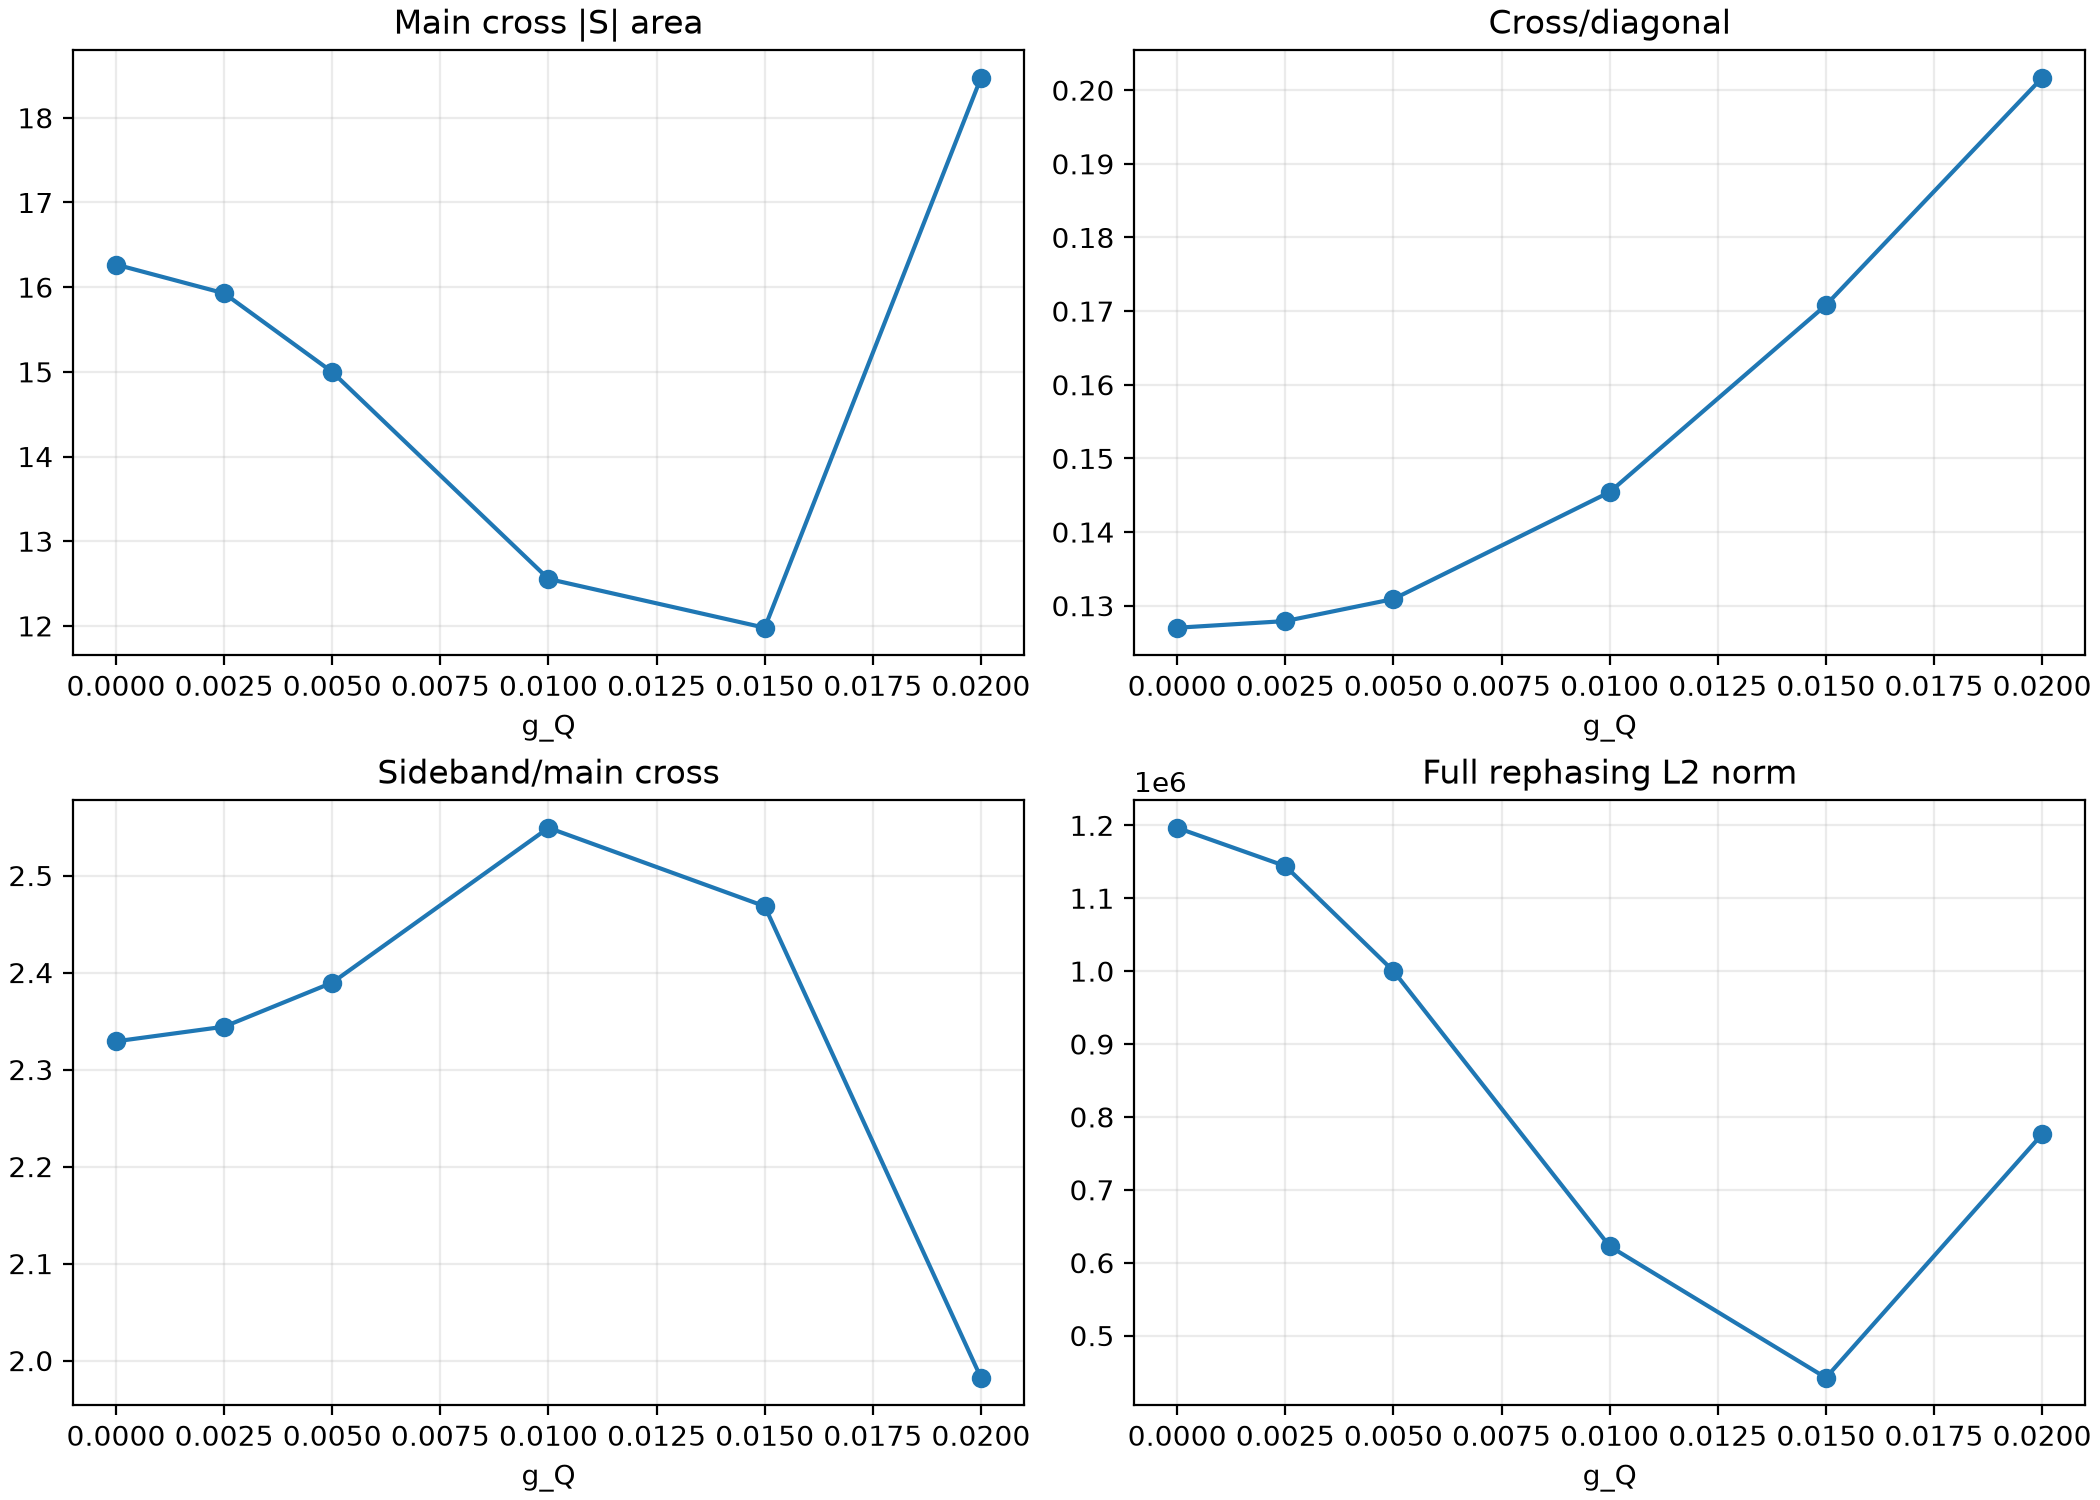
\includegraphics[width=0.95\linewidth]{Analysis/step6_gQ_scan_metrics.png}
\caption{Scan of $g_Q$ at fixed $V_{BD}^{\mathrm{static}}=0.02$ and
$\omega_Q=0.035$ eV.}
\end{figure}

\begin{figure}[h]
\centering
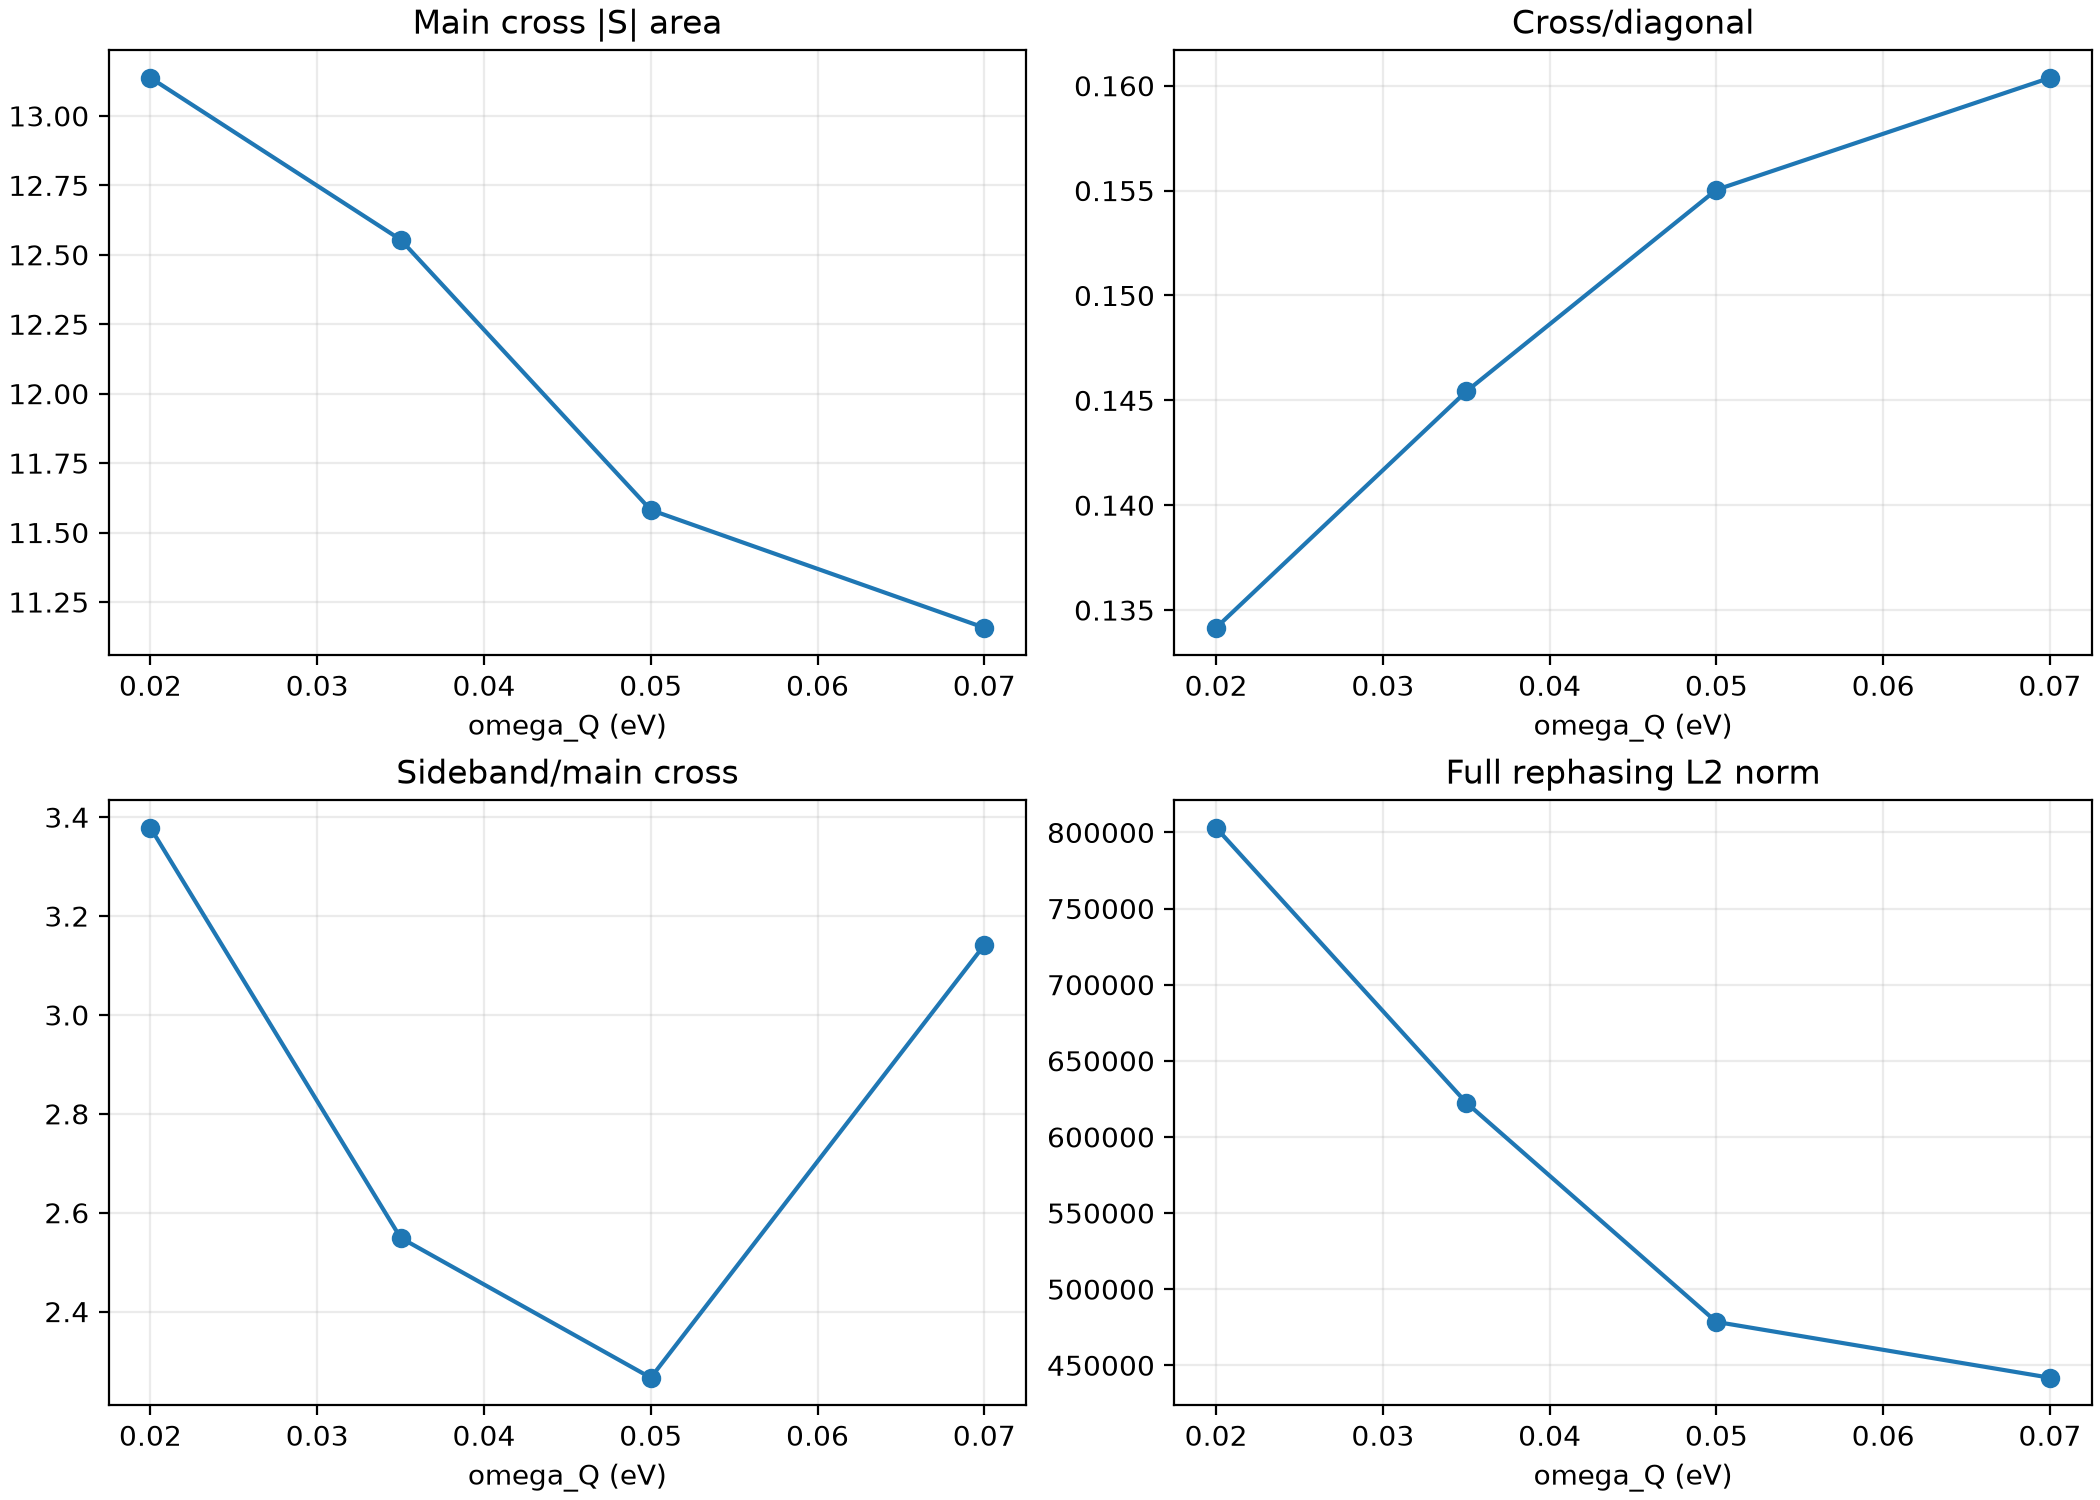
\includegraphics[width=0.95\linewidth]{Analysis/step6_omegaQ_scan_metrics.png}
\caption{Scan of $\omega_Q$ at fixed $V_{BD}^{\mathrm{static}}=0.02$ and
$g_Q=0.010$.}
\end{figure}

\section{Validation outcome}
The $g_Q$ criterion passes.  Nonzero $g_Q$ produces a clear change relative to
the static $g_Q=0$ reference, with fixed $V_{BD}^{\mathrm{static}}$.  Therefore
the spectral change cannot be attributed to scalar bright-dark mixing alone.
The most robust indicators in this scan are the full rephasing norm and the
cross/diagonal ratio.

The $\omega_Q$ criterion also passes at the level of trend sensitivity.  The
sideband/main-cross ratio varies substantially across the scan, and the main
cross-window area, cross/diagonal ratio, and full rephasing norm also change
with $\omega_Q$.  The sideband metric should not yet be read as a precise
phonon-energy measurement because it is based on finite windows rather than a
peak-fitting procedure.

Overall, Step 6 confirms that the dynamic phonon coordinate produces spectral
information beyond the scalar $V_{BD}^{\mathrm{static}}$ channel.  The next
technical refinement should be a more targeted sideband or peak-tracking
analysis, especially if $\omega_Q$ is to be extracted quantitatively.

\end{document}
